%    minted language=cpp,

%%%%%%
%%%%%%%%%%%%%%%%%%%%%%%%%%%%%% Title Page Info %%%%%%%%%%%%%%%%%%%%%%%%%%%%%%%%%%%%%%%%%%%
%%%%%%%%%%%%%%%%%%%%%%%%%%%%%%%%%%%%%%%%%%%%%%%%%%%%%%%%%%%%%%%%%%%%%%%%%%%%%%%%%%%%%%%%%%

\documentclass[aspectratio=169,compress]{beamer}
\mode<presentation> 

\usetheme{Warsaw}
\usecolortheme[rgb={0.93,0.50,0.93}]{structure}


\usepackage[algosection,lined]{algorithm2e}
\usepackage{minted}
\usepackage{tcolorbox}
\tcbuselibrary{minted}


% define
%\usepackage{beamerouterthememiniframes} % Para los puntitos 
\setbeamertemplate{footline}[frame number]{}

% include packages
\usepackage{subfigure}
\usepackage{multicol}
\usepackage{amsmath}
\usepackage{epsfig}
\usepackage{graphicx}
\usepackage[all,knot]{xy}
\usepackage{algorithmic}
\xyoption{arc}
\usepackage{url}
\usepackage{multimedia}
\usepackage{hyperref}
\usepackage{tikz}

\usepackage{pgfpages}
\setbeameroption{hide notes} % Only slides
%\setbeameroption{show only notes} % Only notes
%\setbeameroption{show notes on second screen=right} % Both




%\title{20 proyectos de la línea de sistemas inteligentes de la maestría en ingeniería de la UPV: aplicaciones en el área de salud, agroindustria, seguridad y educación}
%\title{Proyectos selectos de visión por computadora y aprendizaje automático del Laboratorio de Sistemas Inteligentes de la UPV} % TecMTY
%\title{Fundamentos de VR-AR mediante aplicaciones Gráficas 3D en Android utilizando OpenGL- Parte I\\ \large 3er Foro Nacional de Tecnologías de la Información y Sistemas Computacionales} % UPP
%\title{Aplicaciones de Realidad Aumentada y Realidad Virtual de la Universidad Polit\'ecnica de Victoria} % UPP
\title{Aplicaciones de Realidad Aumentada y Realidad Virtual} % UPP

\author{Dr. Marco Aurelio Nu\~no Maganda}
\institute{Universidad Politécnica de Victoria\\ Laboratorio de Sistemas Inteligentes \\
mnunom@upv.edu.mx  \vspace{.25cm} }

\date{Marzo de 2026}
%\textbf{nmaganda@ccc.inaoep.mx}

%%%%%%%%%%%%%%%%%%%%%%%%%%%%%%%%%%%%%%%%%%%%%%%%%%%%%%%%%%%%%%%%%%%%%%%%%%%%%%%%%%%%%%%%%%
%%%%%%%%%%%%%%%%%%%%%%%%%%%%%% Begin Your Document %%%%%%%%%%%%%%%%%%%%%%%%%%%%%%%%%%%%%%%
%%%%%%%%%%%%%%%%%%%%%%%%%%%%%%%%%%%%%%%%%%%%%%%%%%%%%%%%%%%%%%%%%%%%%%%%%%%%%%%%%%%%%%%%%%

 

%\usepackage[backend=biber,maxcitenames=50,maxbibnames=50,sorting=ydmdddnt]{biblatex}
\usepackage[backend=biber,maxcitenames=50,maxbibnames=50,sorting=none]{biblatex}






%\renewrobustcmd{\mkbibfootnote}{\normalsize\footnotemark\footnotetext}
\setbeamerfont{footnote}{size=\tiny}






\newcommand{\ArchivoPrincipal}{Todos}
\newcommand{\ArchivoSecundario}{Bibliografia}


%Append keywords to identify different bibliography entries.
\DeclareSourcemap{
  \maps[datatype=bibtex, overwrite]{
    \map{
      \perdatasource{\ArchivoPrincipal.bib}
      \step[fieldset=KEYWORDS, fieldvalue=primary, append]
    }
    \map{
      \perdatasource{\ArchivoSecundario.bib}
      \step[fieldset=KEYWORDS, fieldvalue=secundary, append]
    }    
  }
}


\addbibresource{\ArchivoPrincipal.bib}
\addbibresource{\ArchivoSecundario.bib}

\usepackage{listings}
 
 \AtBeginSection[]
{
    \begin{frame}
        \frametitle{Outline}
        \tableofcontents[currentsection]
    \end{frame}
}

\makeatletter
\def\@makefnmark{}
\makeatletter
\setbeamertemplate{footnote}{%
  \parindent 1em\noindent
  \raggedright
  *  
  \insertfootnotetext\par
}



\begin{document}

\frame{
	%\titlepage 
	\begin{titlepage}
	\end{titlepage}
	
}



\frame{
\frametitle{Contenido}
\tableofcontents
}



\section[RV]{Conceptos de Realidad Virtual}

\begin{frame}{Realidad Virtual - Antecedente hist\'orico}

\begin{columns}
\begin{column}{0.49\textwidth}


\begin{itemize}
\item Un estereoscopio proporciona im\'agenes separadas para cada ojo mediante lentes individuales, donde cada imagen tiene una variante en el angulo de captura y un desplazamiento horizontal.
\item El cerebro de una persona con una percepción binocular normal de la profundidad al utilizar el estereoscopio ``mezcla'' ambas imagenes para crear una  ``ventana estereoscópica''
\end{itemize}
\end{column}

\begin{column}{0.49\textwidth}

\begin{center}
	\begin{tabular}{cc}
        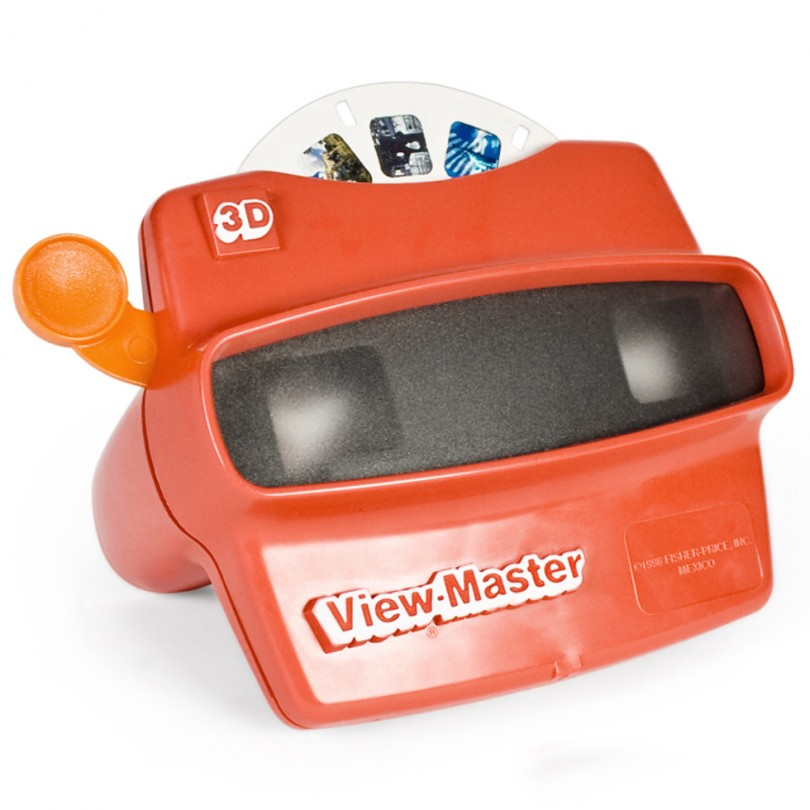
\includegraphics[width=0.45\linewidth]{Figs/view_master_blog-810x810.jpg} &
		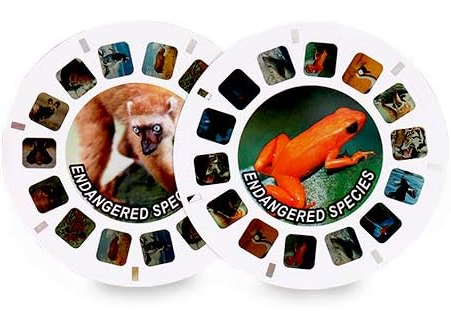
\includegraphics[width=0.45\linewidth]{Figs/DiscosViewMaster.png}    
	\end{tabular}

	\begin{tabular}{cc}
	\centering
        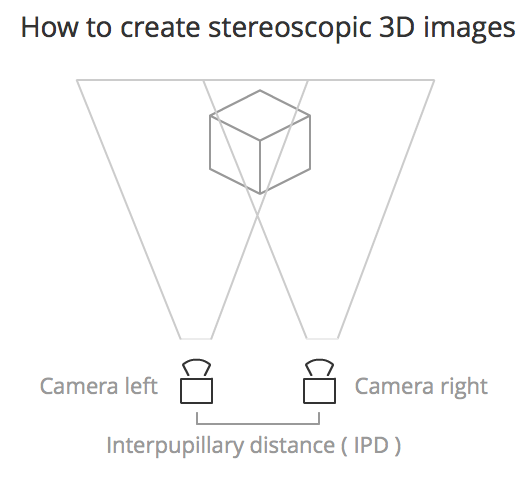
\includegraphics[width=0.49\linewidth]{Figs/VirtualReal1} &
        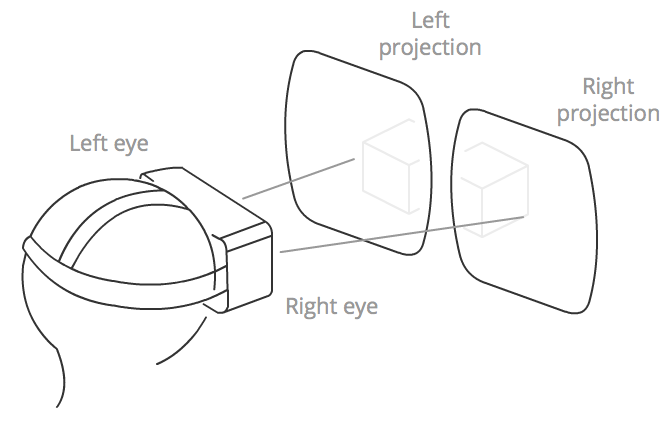
\includegraphics[width=0.49\linewidth]{Figs/VirtualReal2} \\

	\end{tabular}
\end{center}
\end{column}

\end{columns}
	
\end{frame}




\begin{frame}{Realidad Virtual (VR)}
%\begin{block}{Realidad Virtual (VR)} 
		\begin{itemize}
			\item La Realidad virtual (RV) emplea modelos y simulaciones por computadora que permite a una persona interactuar con un entorno visual artificial tridimensional (3D)
			\item En un formato típico de RV, un usuario lleva un casco con una pantalla estereoscópica para ver imágenes animadas de un entorno simulado
			\item El dispositivo m\'as econ\'omico para aplicaciones de RV es un tel\'efono inteligente 
		\end{itemize}
    \begin{center}
	\begin{tabular}{ccc}
    	\centering
		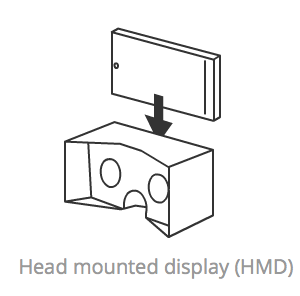
\includegraphics[width=0.25\linewidth]{Figs/MobileVR2} & 
        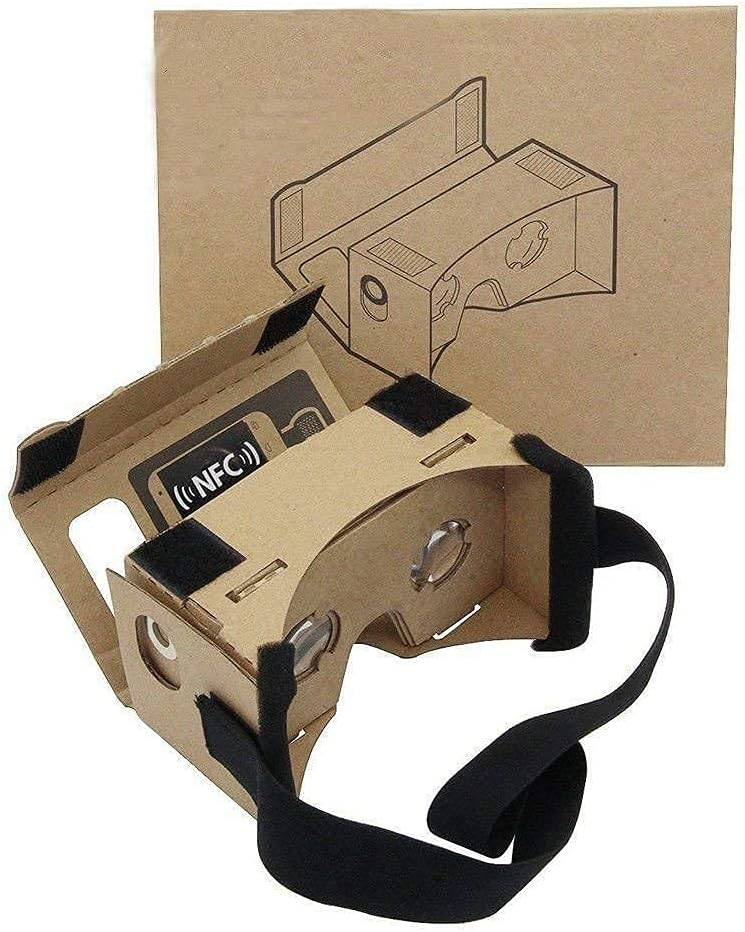
\includegraphics[width=0.19\linewidth]{Figs/CardBoard} & 		
        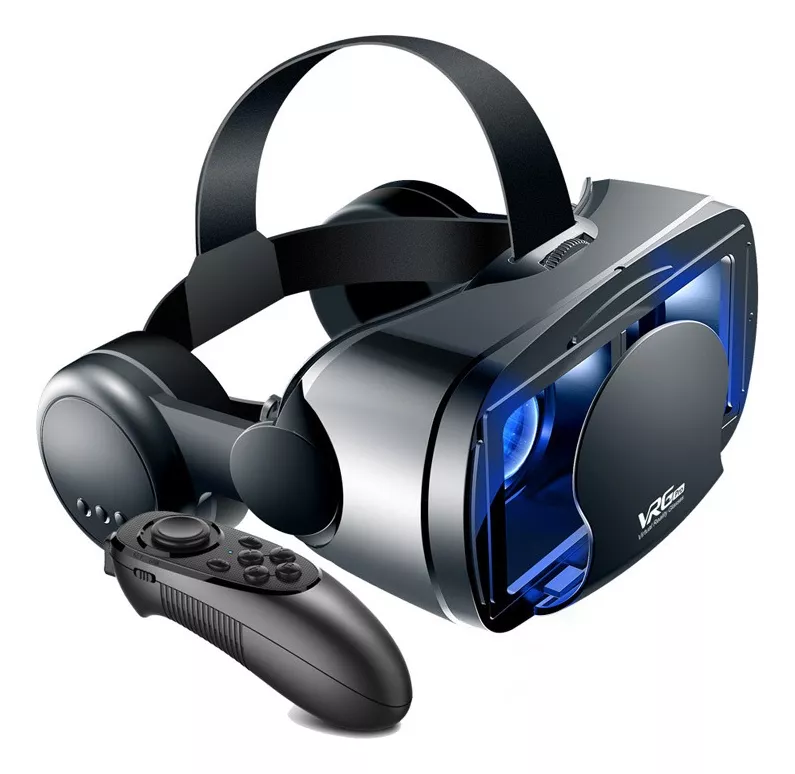
\includegraphics[width=0.19\linewidth]{Figs/VRGPro} 		
	\end{tabular}
		 \end{center}
%\end{block} 
\footnotetext{\url{https://reference.codeproject.com/book/dom/webvr_api/webvr_concepts}}
\end{frame}


\begin{frame}{Costos de Dispostivos HeadSets para VR}
\begin{columns}
\begin{column}{0.49\textwidth}
\begin{itemize}
\item Meta Quest 3 (499 USD)
\item Sony PlayStation VR2 (599 USD)
\item Meta Quest Pro (900 USD)
\item Valve Index VR Kit (1350 USD)
\item HTC Vive Pro 2 (1400 USD)
\end{itemize}

\begin{center}
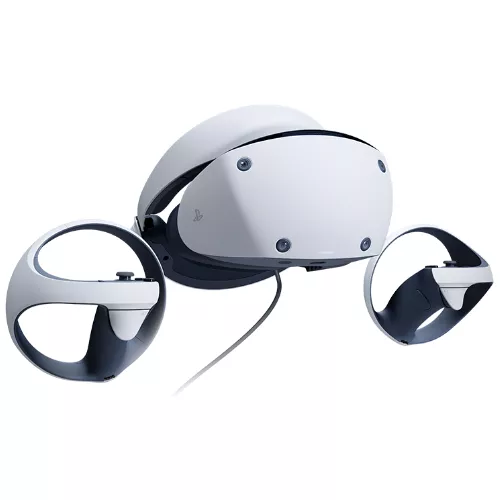
\includegraphics[width=0.75\textwidth]{Figs/sony.png}
\end{center}
\end{column}
\begin{column}{0.49\textwidth}
\begin{center}
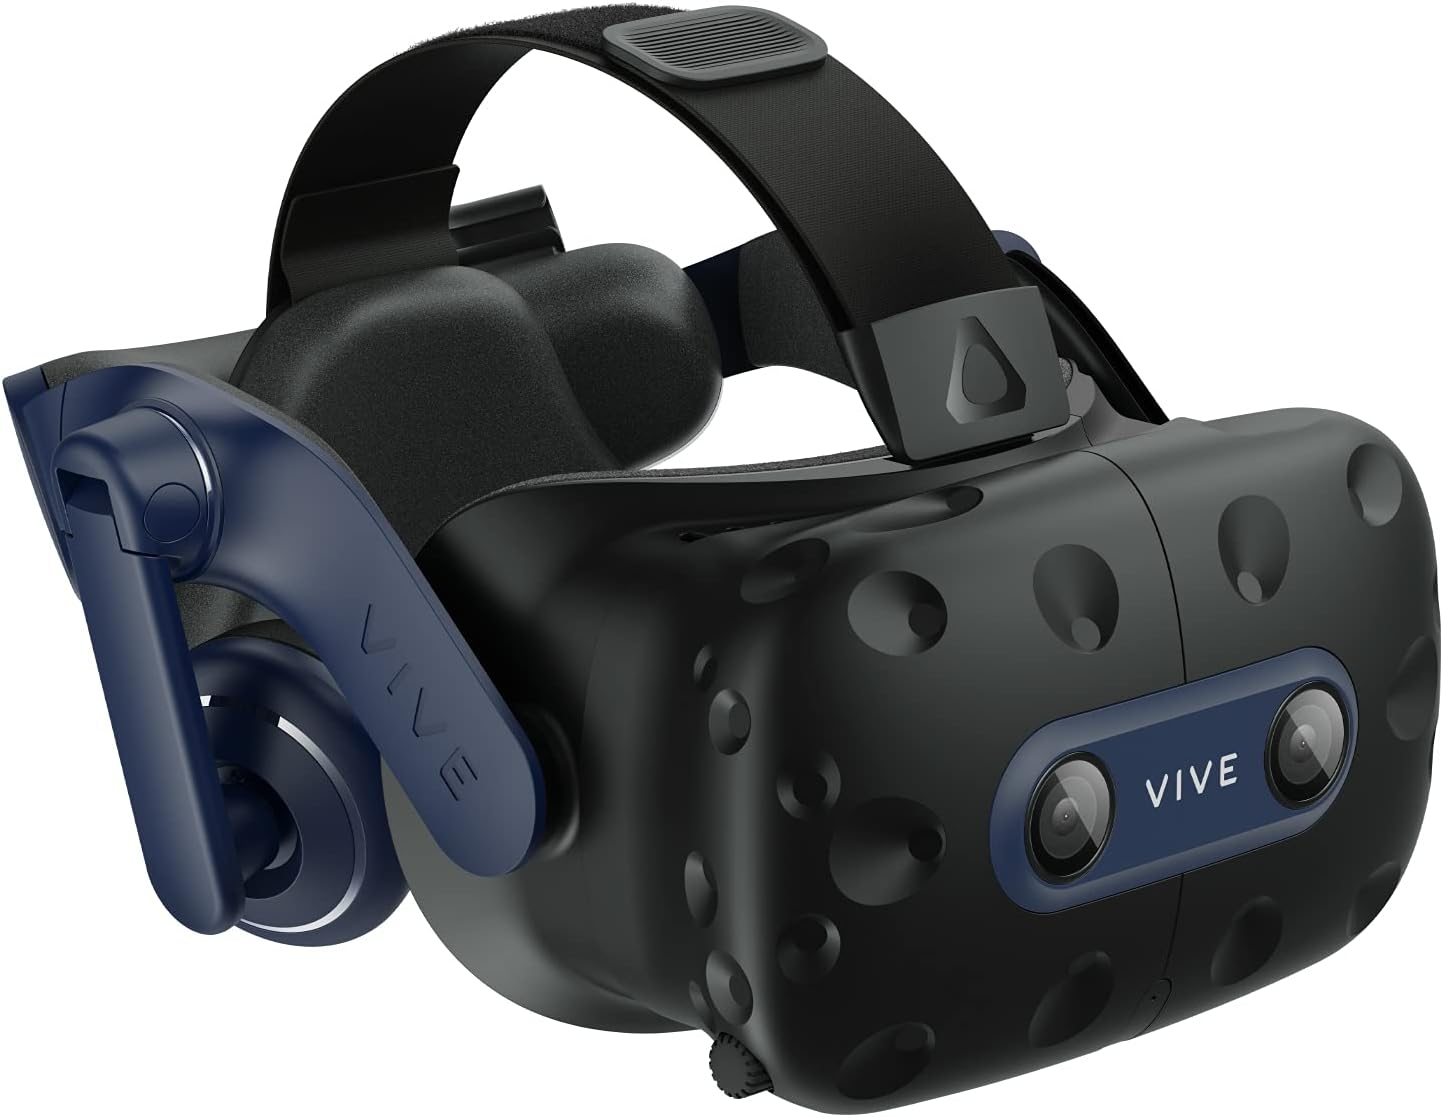
\includegraphics[width=0.75\textwidth]{Figs/HTC.jpg}\\
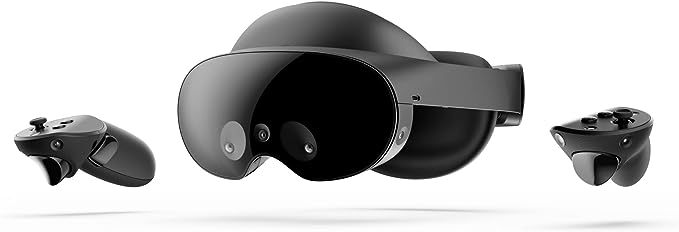
\includegraphics[width=0.95\textwidth]{Figs/MetaPro.jpg}
\end{center}
\end{column}
\end{columns}
\end{frame}


\begin{frame}{Relación entre RV - Teléfonos Inteligentes}
Los teléfonos inteligentes son una de las principales plataformas para sistemas de realidad virtual (VR):  
\begin{itemize}
\item Tienen hardware avanzado (cámaras, sensores de movimiento, procesadores gráficos) que permiten ejecutar experiencias inmersivas de VR sin necesidad de equipos especializados.  
\item Existen accesorios como \textbf{gafas VR para móviles} (ej. Google Cardboard, Samsung Gear VR) que convierten un teléfono en un visor de realidad virtual.  
\item Existen herramientas para crear apps de  RV
\item Muchas aplicaciones combinan AR con inteligencia artificial para ofrecer experiencias interactivas y personalizadas.  
\item Gran cantidad de aplicaciones prácticas
\end{itemize}
\end{frame}


\section[PRV]{Recorridos Virtuales}

\begin{frame}{Recorridos Virtuales y Uso de Teléfonos Inteligentes}

\textbf{¿Qué son los recorridos virtuales?}
\begin{itemize}
    \item Son representaciones digitales interactivas de espacios reales o simulados.
    \item Permiten explorar lugares de forma remota mediante imágenes 360°, video o entornos 3D.
    \item Se utilizan en turismo, educación, bienes raíces y museos.
\end{itemize}

\vspace{0.5cm}

\textbf{¿Cómo ayudan los teléfonos inteligentes?}
\begin{itemize}
    \item \textbf{Portabilidad:} Acceso a recorridos en cualquier momento y lugar.
    \item \textbf{Sensores integrados:} Uso de giroscopio y acelerómetro para navegación inmersiva.
    \item \textbf{Cámara:} Captura de imágenes 360° para crear contenido.
    \item \textbf{Realidad Virtual/Aumentada:} Integración con apps para experiencias más interactivas.
    \item \textbf{Conectividad:} Acceso a contenido en línea y plataformas colaborativas.
\end{itemize}

\end{frame}

\begin{frame}{Recorridos Virtuales Desarrollados en la UPV}
\textbf{}
\begin{itemize}
\item Los recorridos son proyectos de materia (\textit{Programación Móvil o Desarrollo de Aplicaciones Móviles} según la generación). 
\item Principalmente desarrollados por estudiantes de la carrera de \textbf{Ingeniería en Tecnologías de la Información (ITI)/Ingeniería en Tecnologías de la Información e Innovación Digital (ITIID)} de la \textit{Universidad Politécnica de Victoria}.
\item Algunos han pasado por varios grupos de estudiantes, quienes los mejoran y obtienen la siguiente versión.  
\item Se seleccionó desarrollar una Aplicación Nativa por encima de una plataforma por cuestión de desempeño. 
\item Específicamente, se seleccionó Android debido a:
\begin{itemize}
\item Disponibilidad en los teléfonos de los estudiantes 
\item EL IDE para desarrollo (Android Studio) es gratis.  
\item El bajo costo para cargar la app en la tienda de aplicaciones.  
\end{itemize}

\end{itemize}
\end{frame}

 
\begin{frame}{Acerca de los Recorridos Virtuales desarollados}
\textbf{Ventajas}
\begin{itemize}
    \item No requerir de un dispositivo especializado (de alto costo) ya que solo se necesita un teléfono inteligente.
    \item El código abierto permite que una comunidad de desarrolladores aporte mejoras.
	\item Puede ser ejecutado y una diversidad de modelos. 
\end{itemize}

\textbf{Desventajas}
\begin{itemize}
    \item El telefóno inteligente no puede ser utilizado para otras actividades durante el DEMO. 
    \item El desempeño puede estar limitado por las prestaciones del teléfono inteligente.
    \item Se requiere de otros aditamentos (Control de Videojuego y Adaptador para Teléfono Inteligente).
\end{itemize}

\end{frame}


\begin{frame}{Material requerido}
Dispositivos:
\begin{itemize}
\item Un teléfono inteligente con Sistema Operativo Android y soporte para realidad virtual.
\item Un control de XBox (o Genérico) con interfaz Bluetooth\tm. Este dispositivo debe estar vinculado con el smartphone. 
\item Una carcasa para realidad virtual. 

\end{itemize}

Demos disponibles:
\begin{itemize}
\item Recorrido Virtual de la UPV.
\item Museo de Historia Regional de Tamaulipas.
\item Pinacoteca de Ciudad Victoria, Tamaulipas.
\item Casa del Arte de Ciudad Victoria, Tamaulipas.
\end{itemize}
\end{frame}


%\input{2021_RecorridoUPV/RecorridoUPV.tex} % Actualizacion

\renewcommand{\Folder}{2025_RecorridoUPV}
\renewcommand{\EntradaBibtex}{2025_RecorridoUPV}

\begin{frame}{\citetitle{\EntradaBibtex} \footnotemark[1] (1)}
\begin{columns}
	\begin{column}{0.60\textwidth}
		\begin{itemize}
			\item Primer aplicación de realidad virtual solicitada a estudiantes en la UPV. 
			\item Ha pasado por 4 generaciones hasta la versión actual.
            \item Proyecto destacado ya que se utiliza para ferias vocaciones y eventos de promoción.
		\end{itemize}
	\end{column}
	\begin{column}{0.40\textwidth}
		\begin{center}
			
\includegraphics[width=0.98\textwidth]{\Folder/figs/img1}
		\end{center}
		 \begin{center}
		     
\includegraphics[width=0.98\textwidth]{\Folder/figs/img2}
		 \end{center}

	\end{column}
	
\end{columns}

%\end{block} 
\footnotetext[1]{\fullcite{\EntradaBibtex}}
\end{frame}


\begin{frame}{\citetitle{\EntradaBibtex}  (2)}
\begin{columns}
	\begin{column}{0.48\textwidth}
		\begin{itemize}
			\item Se modelan 4 edificios de la UPV (actualmente hay 6). 
			\item Con el control de XBox es posible moverse en el entorno virtual.
			\item Los sensores del smartphone actualizan la vista en base a la posición de la cabeza del usuario.
		\end{itemize}


	\end{column}
	\begin{column}{0.48\textwidth}
		\begin{center}
			
\includegraphics[width=0.98\textwidth]{\Folder/figs/img3}
		\end{center}
		 \begin{center}
		     
\includegraphics[width=0.98\textwidth]{\Folder/figs/img4}
		 \end{center}

	\end{column}
	
\end{columns}

%\end{block} 
%\footnotetext[1]{\fullcite{\EntradaBibtex}}
\end{frame}

 % Actualizacion
\input{2023_MuseoRegional_Virtual/MuseoRegional.tex}
\input{2024_Pinacoteca_Virtual/PicacotecaVirtual.tex}

%\renewcommand{\EntradaBibtex}{PinacotecaVirtual_2024}
\renewcommand{\Folder}{2025_RecorridoVirtualCasaArte}
\renewcommand{\EntradaBibtex}{2025_RecorridoVirtualCasaArte}


\begin{frame}{\citetitle{\EntradaBibtex}$^*$ (1)}
\begin{block}{Motivación} 
Los recorridos virtuales ofrecen una herramienta valiosa para explorar y experimentar entornos tridimensionales, tanto en contextos educativos como recreativo.
\begin{itemize}
\item Se implementó una aplicación móvil para explorar de manera interactiva la case del Arte en Ciudad Victoria Tamaulipas. 
%\begin{itemize}
%\item Permite al usuario llevar el conteo de sentadillas, tanto se las hace de frente como de lado.
%\item Debe ubicar el dispositivo a una distancia de 80 cm. Si el ejercicio no es bien realizado, no se contabiliza.
%\end{itemize}
\end{itemize}
\end{block} 
\begin{center}

\includegraphics[width=0.48\linewidth]{\Folder/figs/CasaArte.jpg}
\end{center}
\footfullcite*{\EntradaBibtex}
\end{frame}


\begin{frame}{\citetitle{\EntradaBibtex} (2)}
%\begin{block}{Pantallas Principales} 

\begin{columns}
% Column 1
\column{.99\linewidth}



\begin{center}
	\begin{tabular}{cc}
		
\includegraphics[width=0.45\linewidth]{\Folder/figs/3d_1.jpeg} &
		
\includegraphics[width=0.45\linewidth]{\Folder/figs/3d_3.jpeg} \\
		
\includegraphics[width=0.45\linewidth]{\Folder/figs/3d_5.jpeg} &
 		
\includegraphics[width=0.45\linewidth]{\Folder/figs/3d_8.jpeg} \\
	\end{tabular}
\end{center}



%\column{.5\linewidth}
%\begin{center}
	%\begin{tabular}{cccc}
	%	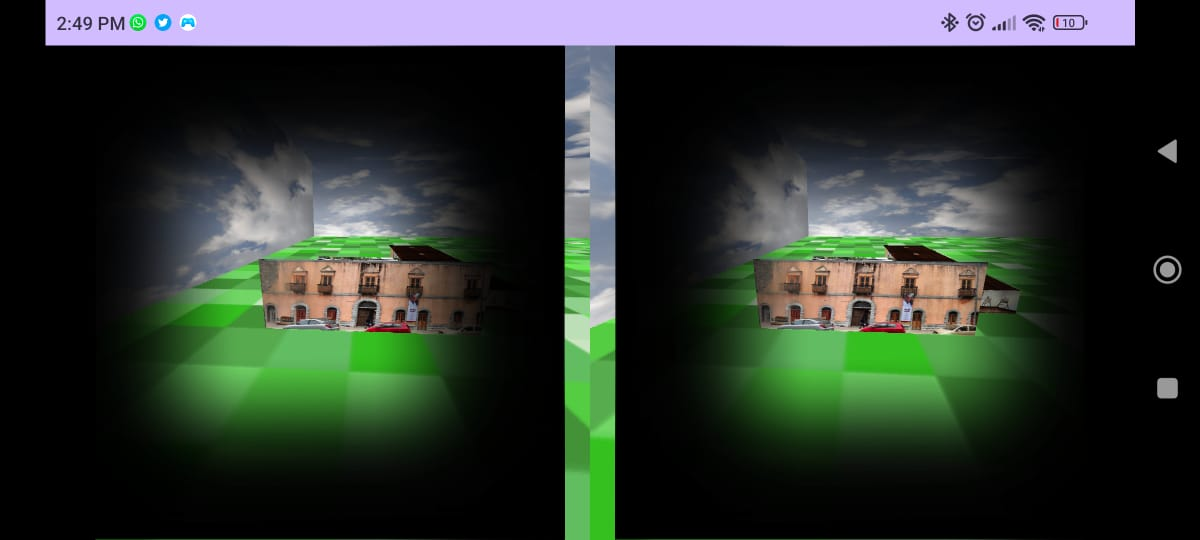
\includegraphics[width=0.40\linewidth]{2024_Pinacoteca_Virtual/PlanoGeneral.jpeg} &
 	%	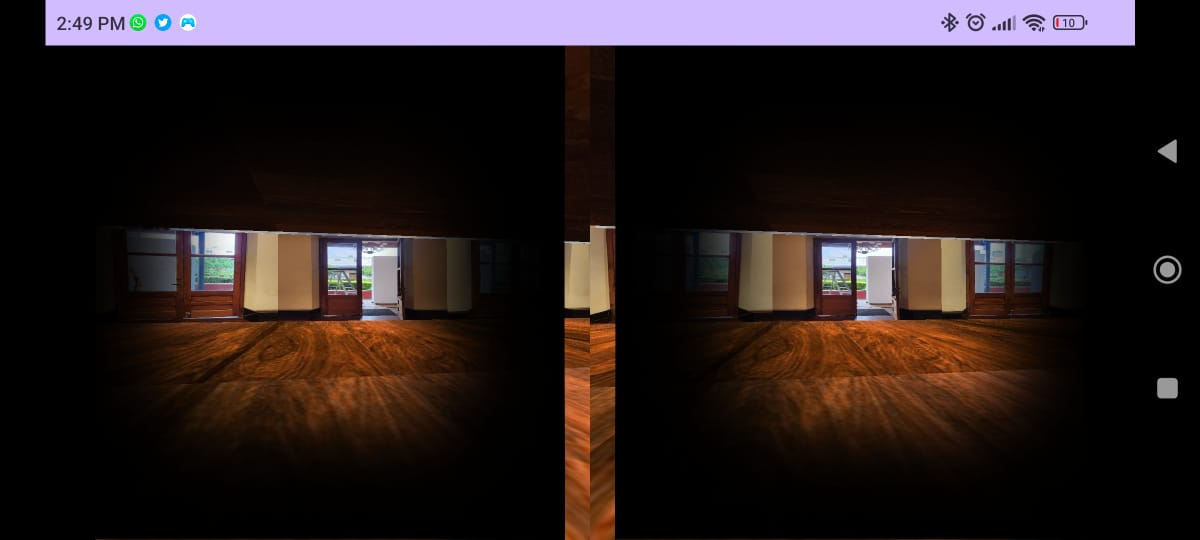
\includegraphics[width=0.40\linewidth]{2024_Pinacoteca_Virtual/Salida_SalonExhibiciones.jpeg} \\
%	\end{tabular}
%\end{center}


\end{columns}
\end{frame}






\section[CP1]{Conclusiones }
\begin{frame}{Conclusi\'on y Áreas de Oportunidad}
\begin{itemize}
\item Se presentaron conceptos relacionados con la RV. 
\item Se describen las herramientas requeridas para interactuar con los demos realizados. 
\item Se describen los demos implementados. Es posible que os asistentes interactúen con los demos presentados si se solicita extender esta presentación de manera presencial.
\end{itemize}
\end{frame}



\end{document}

